\section{Experiments}

\subsection{System setup}
The system is consisted of a robot mounted with a motorized needle driver, a robot mounted with a stent graft sewing mandrel, a fixed position needle driver, a curved needle and a stereo camera (Figure~\ref{}). The system workflow is as below:

\begin{enumerate}
\item{1}: Needle driver holding needle root
\item{2}: Vision system detect the needle pose relative to the needle driver
\item{3}: New robot trajectory is generated according to the needle pose
\item{4}: Needle driver approaching mandrel
\item{5}: Needle piercing into the fabric and the tip piercing out of fabric
\item{6}: Needle driver releasing the needle root, approaching the needle tip
\item{7}: Needle driver griping the needle tip and piercing the whole needle out of fabric
\item{8}: Needle driver bringing the needle to the second needle driver
\item{9}: The second needle driver griping the middle of the needle, the first needle driver griping the root of the needle
\end{enumerate}

% Stereo system
The stereo system is consisted of two identical Logitch HD cameras. The cameras are fixed on a tripod and are about 10$cm$ distance from each other. Stereo calibration and points triangulation are done by use the OpenCV. The calibration accuracy is measured by using the triangulation results to measure distance between two feature points on the camera view. The error is 0.89 $mm$.

The camera frame is registered to the robot frame by hand eye calibration. During the calibration, a key dot pattern is fixed on a know position of the robot end effector, whose origin is aligned with the end effector origin. The robot moves the key dots around and records the end key dot pattern positions in the robot frame, as well as in the camera frame. The rigid transformation between these two set of positions are computed by using the singular value decomposition technique. This transformation is hence the transformation from the robot frame to the camera frame. We mount the motorized needle driver on the end effector and register the tip pose to the robot. With the result of the hand eye calibration, the needle driver pose in the camera frame is computed.

The needle is initially grip at the very end of the needle driver and we assume that only small displacement of the needle pose will occur during the sewing task. The needle driver tip position is hence used as a prior of the needle position.

\subsection{Human demonstration}
For teaching robot the sewing task, we carry out four demonstrations. All demonstrations starts from the same position and sew the same slot on the mandrel. To control the quality of the stitches, across all demonstrations the needle pierces in at the same location and pierces out at the same location. At the beginning of each demonstration, the needle is placed at the same place and normal to the needle driver. Hence the needle pose in the robot frame can be computed accurately.

The demonstrations are segmented into three primitive movements, according to the needle drive open and close even. Figure~\ref{fig:segment} shows one segmentation results. Figure~\ref{fig:demo} shows the demonstrated needle driver trajectories in 3D.

\begin{figure}
\centering{
{\includegraphics[width=8cm]{./fig/seg_37.eps}}
\caption{\scriptsize{Segmentation result of human demonstration. The red, green and blue patches label the three segments of the motion}}
\label{fig:segment}
}\end{figure}


\begin{figure*}
\centering{
\subfloat[\scriptsize{Demonstrations of phase 1}] {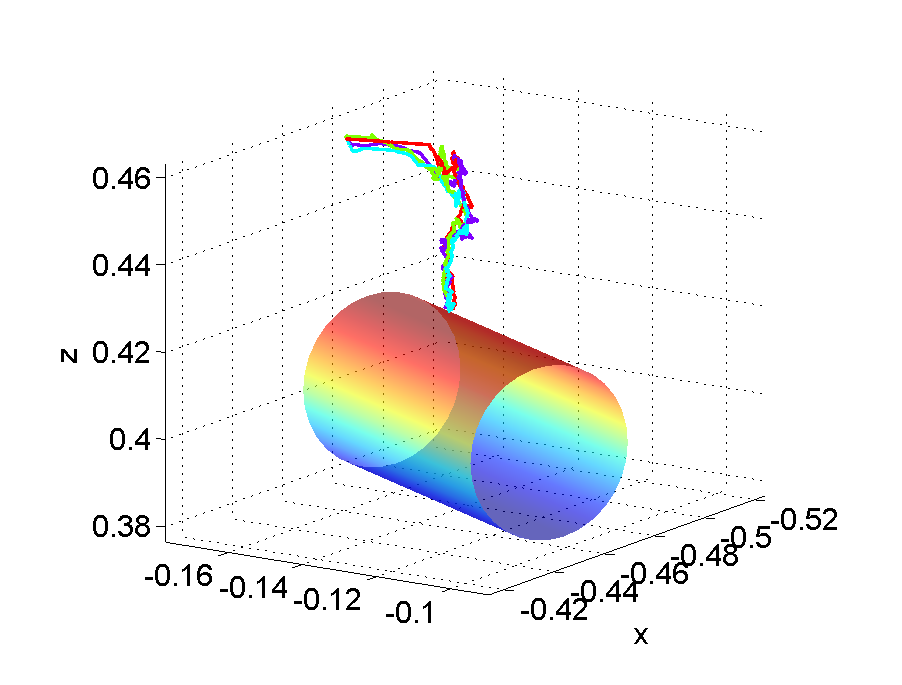
\includegraphics[width=8cm]{./fig/demo_1.eps}}
\subfloat[\scriptsize{Demonstrations of phase 2}]  {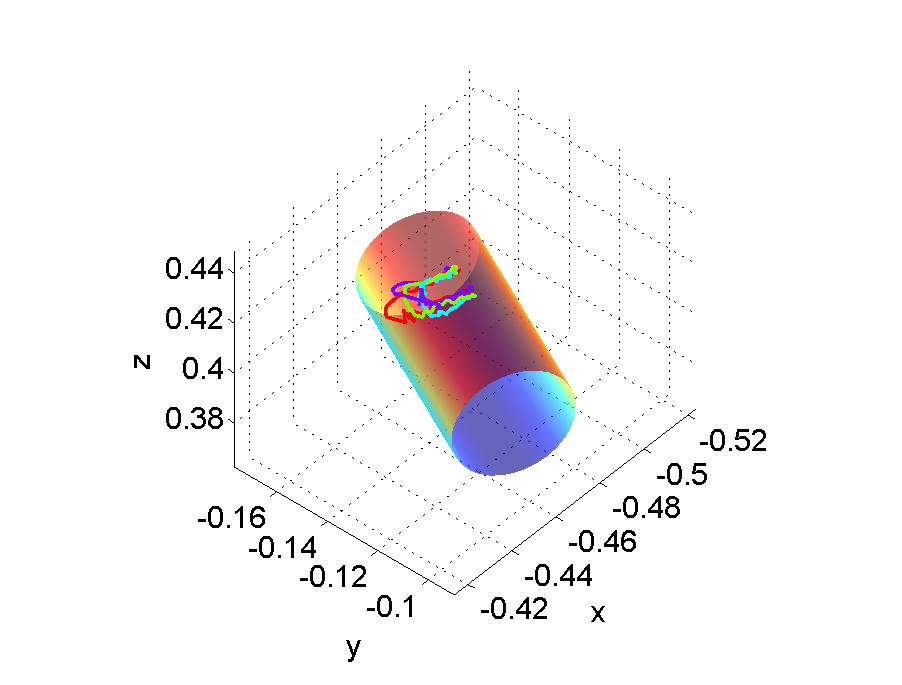
\includegraphics[width=8cm]{./fig/demo_2.eps}}
\\
\subfloat[\scriptsize{Demonstrations of phase 3}]  {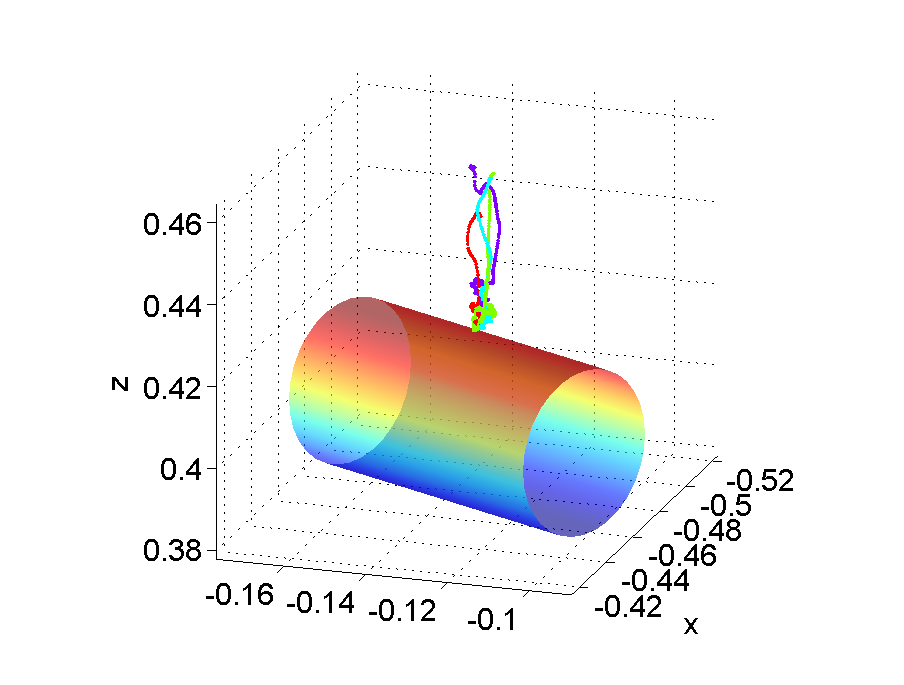
\includegraphics[width=8cm]{./fig/demo_3.eps}}
\subfloat[\scriptsize{Learnt trajectory of phase 1,2 and 3}]  {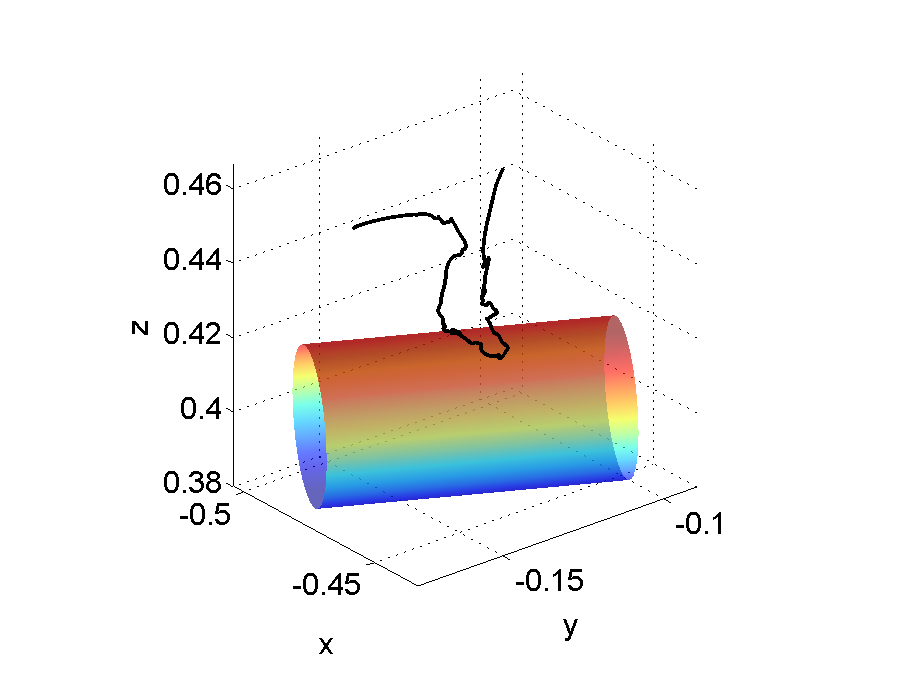
\includegraphics[width=8cm]{./fig/learn_123.eps}}
\caption{\scriptsize{Needle driver trajectories of human demonstrations and the learnt result. The cylinder represents the mandrel}}
\label{fig:demo}
}\end{figure*}

\subsection{Learning}
GMM is used to learn model for each phase. Figure~\ref{fig:GMR} shows a 2D projection of the build model of each phase. It can be seem from the model that the three phases have different charactoristics. Phase one has small variance from the beginning to the end, as all the movements start from the same point and pierce into the same location. The piercing movements are the same in order to produce similar stitches. Phase two has larger variance compare to phase one, as the needle is detached with the robot and the robot movement has less constraints. Phase three has small variance at the beginning, when the robot needs to pull out the needle from the same location, and has large variance once the needle is pulled out from the fabric. These show that the GMM can effectively capture the constraints at each phase and hence generate proper trajectories for the robot to complete the task.

\begin{figure*}
\centering{
\subfloat[\scriptsize{Phase 1}] {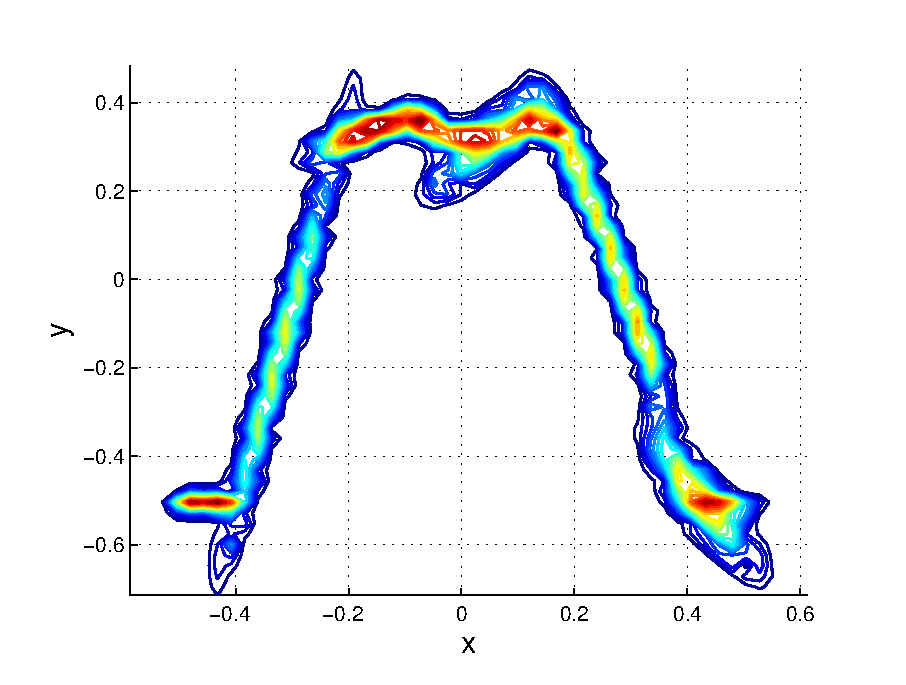
\includegraphics[width=6cm]{./fig/gmm_contour1_1-2.eps}}
\subfloat[\scriptsize{Phase 2}]  {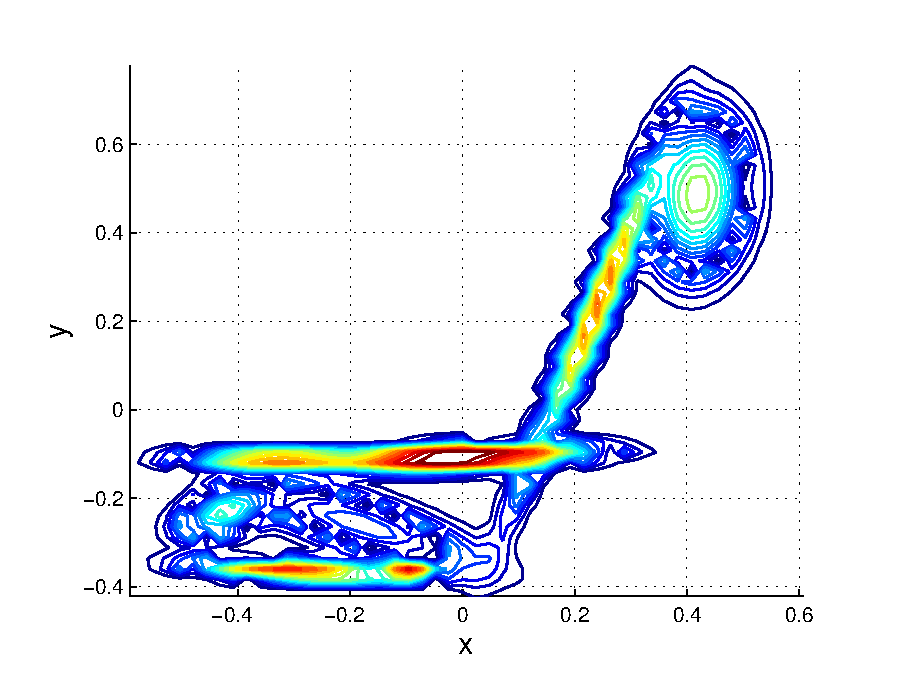
\includegraphics[width=6cm]{./fig/gmm_contour2_1-2.eps}}
\\
\subfloat[\scriptsize{Phase 3}]  {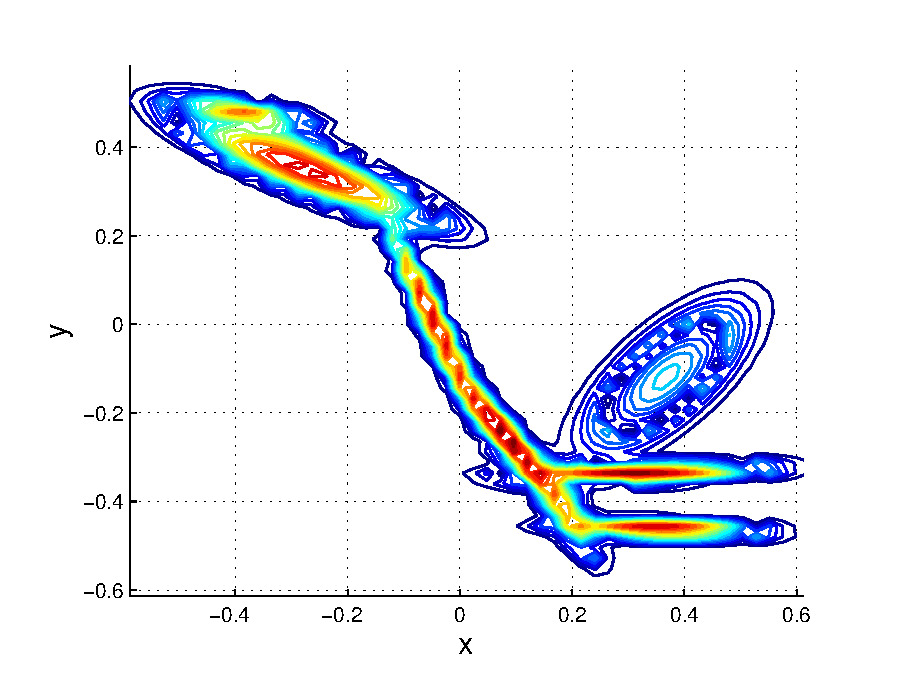
\includegraphics[width=6cm]{./fig/gmm_contour3_1-2.eps}}
\caption{\scriptsize{2D representation of the learnt models of different phases.}}
\label{fig:demo}
}\end{figure*}


\subsection{Task execution}
